\section{Estrutura} \label{Secao Estrutura}

O suporte ou rolo, como é comumente chamado pelos ciclistas, tem como papel transformar uma bicicleta normal em uma do tipo ergométrica, uma vez que este suporte irá levantar a roda traseira ou as duas, dependendo do modelo, fazendo com que a bicicleta permaneça fixa no local em que se realiza a atividade física.  Existem atualmente no mercado, quatros tipos mais comuns de rolos de treinamento:
\begin{enumerate}
    \item Rolo de equilíbrio
    \item Rolo de treinamento de resistência magnética
    \item Rolo de treinamento com resistência de fluidos
    \item Rolo de treinamento comum
\end{enumerate}

Na figura \ref{fig:rolos} a seguir, podemos visualizar na sequência, os quatros tipos:

\begin{figure}[h]
    \centering
    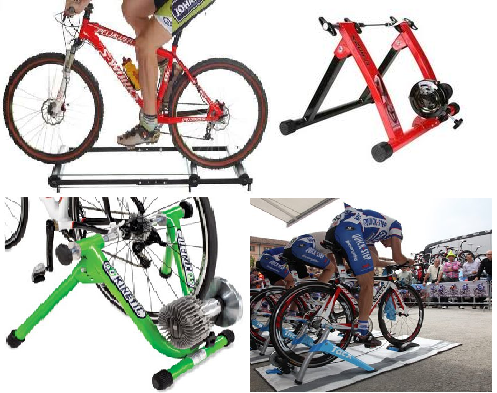
\includegraphics[width=0.7\textwidth]{figuras/rolos.png}
    \caption{Estrutura}
    \label{fig:rolos}
\end{figure}

Fazendo-se um levantamento das necessidades de projeto, o rolo escolhido para gerar a pedalada do ciclista foi o rolo de treinamento comum, pois sua construção é simples e barata se comparada aos outros modelos. 

Como o produto proposto, deverá fazer uma transforma eletromecânica, não se fez necessário o uso do rolo no suporte,  o pneu será retirado, e uma correia será acoplada na roda, para que essa rotação seja transmitida para o alternador. Feita essas especificações necessárias para a sua construção, o seu desenho em CAD foi feito. 

Para a construção física do suporte, tiramos como base, a teoria de estruturas em treliça, o qual é formado por cinco ou mais unidades triangulares, construídas com elementos retos, cujas extremidades são ligadas em pontos conhecidos como nós. Para as forças externas e reações consideram-se, de forma simplificada, aplicadas nestes mesmos nós. Onde, o bom desempenho de uma treliça é garantido se as cargas são aplicadas nas juntas ou nós. A forma como será montado o suporte, as solicitações se encontraram aplicadas sobres os nós, garantindo assim uma estrutura rígida o suficiente e estável para ser acoplada a roda traseira da bicicleta.

\begin{figure}[h]
    \centering
    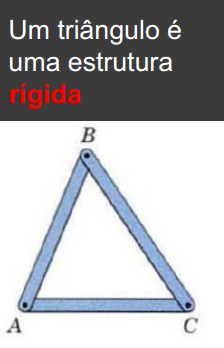
\includegraphics[width=0.5\textwidth]{figuras/trelica.png}
    \caption{Estrutura}
    \label{fig:trelica}
\end{figure}

Uma estrutura simples, de fácil montagem e que possui a rigidez necessária quando se aplicado o material escolhido, para suportar o peso do ciclista. A seguir, segue um diagrama de corpo livre, de uma das estruturas triangulares, que irão formar a base ( ou rolo) sob uma carga de 1KN, estimando-se a que o ocupante não exceda uma carga de 100Kg.

De acordo com as necessidade de projeto, o perfil escolhido foi o do tipo em T de $1"$, em aço 1010. Tal perfil possui as características geométricas necessárias, além de ser barato e possuir baixa densidade, tornando assim a estrutura mais leve. Segue as especificações geométricas do perfil usado:

\begin{figure}[h]
    \centering
    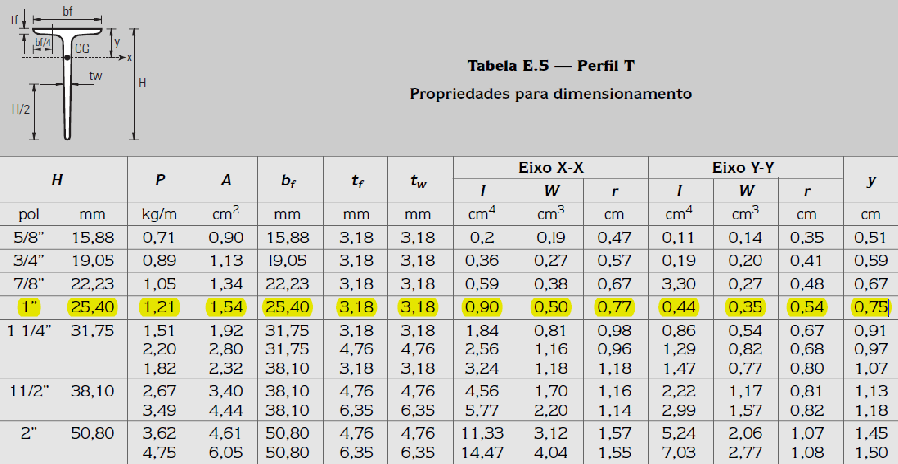
\includegraphics[width=0.8\textwidth]{figuras/perfil_t.png}
    \caption{Estrutura}
    \label{fig:awesome_image}
\end{figure}

Na presente divisão \ref{Secao Estrutura}  a estrutura baseada....na figura \ref{fig:awesome_image} ..... tendo como referencia \cite{shigley2011shigley}.

% \begin{figure}[h]
%    \centering
%    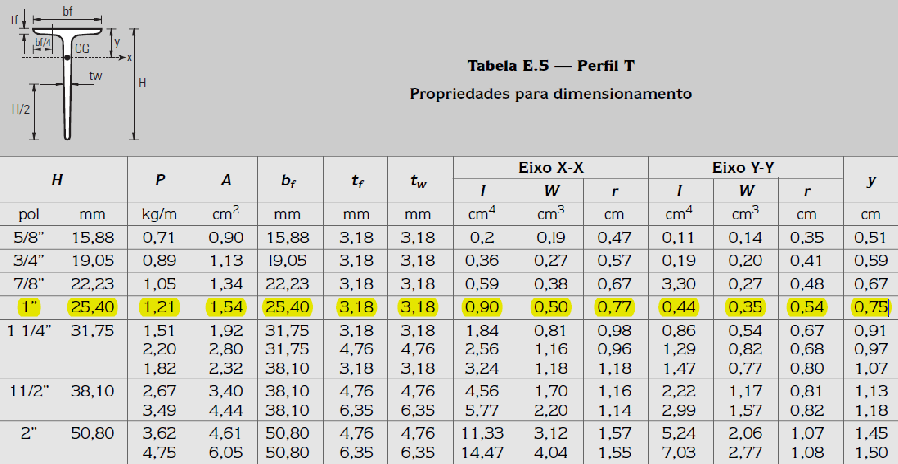
\includegraphics[width=0.8\textwidth]{figuras/perfil_t.png}
%    \caption{Estrutura}
%    \label{fig:awesome_image}
% \end{figure}
